\documentclass[final]{beamer}

\usepackage[orientation=portrait, size=a0, scale=1.4, debug]{beamerposter}
\usepackage{booktabs}
\usepackage{dcolumn}
\usepackage{colortbl}
\usepackage{xcolor}
\usepackage{hyperref}
\usepackage{amsmath}
%\usepackage[absolute, showboxes, overlay]{textpos}
\usepackage[absolute, overlay]{textpos}
\usepackage{calc}
%\usepackage[colorgrid,texcoord]{eso-pic}
\usepackage[bibstyle=numeric]{biblatex}
% \usepackage{enumitem}
% \defaultfontfeatures{Mapping=tex-text}
\usepackage{pifont}
\usepackage{algorithm}
\usepackage[noend]{algpseudocode} 

\usetheme{enziteto}

\addbibresource{../referomnia/referomnia.bib}

\usepackage{blindtext}

\newcommand*\mccol[2]{\multicolumn{#1}{c}{#2}}
\newcommand*\tmccol[2]{\mccol{#1}{\tiny\textsf{#2}}}
\newcommand*\bmccol[2]{\mccol{#1}{\textbf{#2}}}


% 
% custom colors
\definecolor{untractable_red}{RGB}{209, 25, 25}
\definecolor{tractable_green}{RGB}{0, 153, 51}

\newcommand{\cmark}{\ding{51}}%
\newcommand{\xmark}{\ding{55}}

\setbeamertemplate{itemize item}{\raisebox{.21ex}{\hbox{\tiny\textcolor{lacamlilac}{$\boldsymbol{\oplus}$}}\hspace{0pt}}}
\setbeamertemplate{itemize subitem}{\raise .2ex\hbox{\tiny\textcolor{lacamlilac}{$\boldsymbol{\otimes}$}}\hspace{0pt}}
\setbeamertemplate{itemize subsubitem}{\textcolor{lacamlilac}{$\oplus$}}
% \setbeamertemplate{bibliography item}{\hspace{10pt}\raise
%   .2ex\hbox{\tiny\textcolor{lacamlilac}{$\boldsymbol{\oplus}$}}\insertbiblabel}
\setbeamertemplate{bibliography item}{\insertbiblabel}


\setbeamertemplate{headline}{}

% \addbibresource{../referomnia/referomnia.bib}

\title{Towards Representation Learning with Tractable Probabilistic Models}
\author{Antonio  Vergari, Nicola  {Di Mauro} and Floriana Esposito}
\date{}


\begin{document}

\institute{Università degli Studi di Bari}
\department{Dipartimento di Informatica}
\laboratory{LACAM}
\group{Machine Learning}
\institutelogo{
\includegraphics[width=25pt]{figures/unibaba}}
\lablogo{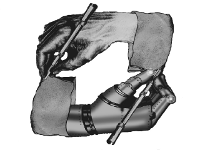
\includegraphics[width=35pt]{figures/lacam}}


% {
%   \setbeamertemplate{headline}{}
%   \setbeamertemplate{footline}{}
%   \begin{textblock}
%     \titlepage
%   \end{textblock}
% }

\newcommand{\hmargin}{20mm}
\newcommand{\vmargin}{20mm}
\textblockorigin{\hmargin}{\vmargin}

\setlength{\TPHorizModule}{1cm}
\setlength{\TPVertModule}{1cm}

%
% TODO: generalize this
\newlength{\posterwidth}
\setlength{\posterwidth}{841mm - 2\hmargin}
\newlength{\posterheight}
\setlength{\posterheight}{1189mm}

\newcommand{\ncols}{3}
\newlength{\colwidth}
\setlength{\colwidth}{\posterwidth/\ncols}

\newlength{\colhpoint}
\setlength{\leftmargini}{30pt}

\begin{frame}{}
  %
  % title
  % \textblockcolour{header}
  \begin{textblock}{58}(0, 0)
    \usebeamerfont{section name}
    \huge
    Towards Representation Learning\\
    with Tractable Probabilistic Models
  \end{textblock}
  %
  % authors
  \begin{textblock}{30}(0, 6.5)
    \usebeamerfont{author}
    \small
    Antonio  Vergari, Nicola  {Di Mauro} and Floriana Esposito
  \end{textblock}
  % 
  % email
  \begin{textblock}{15}(30, 6.5)
    \usebeamerfont{author}
    \small
    \emph{\{firstname.lastname@uniba.it\}}
  \end{textblock}
  %
  % affiliations
  \begin{textblock}{30}(60, 0)
    \usebeamerfont{author}
    \footnotesize
    \begin{minipage}[t]{5cm}
      \vspace{0pt}\hspace{5pt}
      
\includegraphics[width=97pt]{figures/unibaba}
    \end{minipage}\hspace{-15pt}
    \begin{minipage}[t]{15cm}
    \vspace{20pt}
      \flushleft
      University of Bari "Aldo Moro", Italy\\
    \vspace{2pt}
      Department of Computer Science
    \end{minipage}\\[0.75cm]
    \usebeamerfont{author}
    \footnotesize
    \begin{minipage}[t]{5cm}
      \vspace{0pt}
      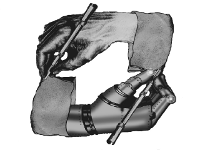
\includegraphics[width=117pt]{figures/lacam}
    \end{minipage}\hspace{-15pt}
    \begin{minipage}[t]{15cm}
      \vspace{23pt}
      \flushleft
      LACAM Laboratory\\
      \vspace{2pt}
      Machine Learning
    \end{minipage}
  \end{textblock}
  
  
  %
  % section 1
  \begin{textblock}{80}(0, 10.5)
    \usebeamerfont{section name}
    Tractable Probabilistic Models
  \end{textblock}
  
  
  \begin{textblock}{25.2}(0, 13)
    \small
    \emph{\textbf{Density estimation}} is the unsupervised task of
    learning an estimator for the joint probability distribution
    $p(\mathbf{X})$ from a set of i.i.d. samples $\{\mathbf
    x^i\}_{i=1}^m$ over RVs $\mathbf{X}$\\[20pt]
    
    Given such an estimator, one uses it to answers
    probabilistic queries about configurations on $\mathbf{X}$,
    i.e. to do \emph{\textbf{inference}}\\[20pt]
    
    Different kinds of inference query kinds:
    \begin{itemize}
    \item $p(\mathbf{X} = \mathbf{x})$ pointwise evidence (EVI) 
    \item $p(\mathbf{E}), \mathbf{E}\subset\mathbf{X}$ marginals (MAR)
    \item $p(\mathbf{Q}|\mathbf{E}), \mathbf{Q},
      \mathbf{E}\subset\mathbf{X}, \mathbf{Q}\cap \mathbf{E}=\emptyset$
      conditionals (CON)
    \item $\arg\max_{\mathbf{q}\sim\mathbf{Q}}p(\mathbf{q}|\mathbf{E})$
      MPE assignments (MPE)
    \item $Z =\sum_{\mathbf{x}\sim \mathbf{X}}\phi(\mathbf{x})$
      partition function (Z)
      \item sampling: generate $\mathbf{x}\sim p(\mathbf{X})$ (SAM)
    \end{itemize}\vspace{20pt}
    
    Good estimators guarantee \emph{exact} and \emph{efficient} inference.

  \end{textblock}
  
  \begin{textblock}{25.2}(27.4, 13)
    \small
    \emph{\textbf{Tractable Probabilistic Models}}  (\textbf{TPMs})
    are density estimators for which some kind of inference is
    \emph{tractable}, i.e. polynomial in the number of r.v.s or their
    domains.\\[20pt]

    Different TPMs guarantee different inference kinds to be tractable.
  \end{textblock}
  
  \begin{textblock}{25.2}(54.8, 13)
    \small
    TPMs can be roughly classified into:
    \begin{itemize}
    \item \textbf{\emph{low-treewidth}} Probabilistic Graphical Models
      (PGMs)($^*$)
    \item \textbf{\emph{computational graphs}} compiling
      $p(\mathbf{X})$ ($^\times$)
    \item \textbf{\emph{neural autoregressive}} models ($^+$) 
    \end{itemize}
     
  \end{textblock}

  \begin{textblock}{52.5}(27.4, 19.5)
    \small
    \begin{minipage}[t]{0.19\linewidth}
      \begin{center}
        \textbf{Tree distributions}~\parencite{Meila2000}~($^*$)\\[20pt]
        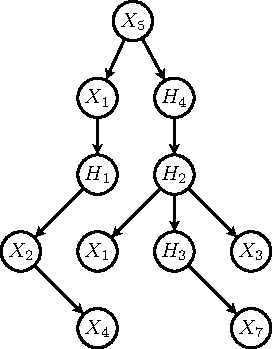
\includegraphics[width=0.65\linewidth]{figures/tree}\vspace{-5pt}
        \begin{minipage}[t]{0.58\linewidth}
          \scriptsize \flushleft 
          \textcolor{tractable_green}{\cmark \textbf{EVI}}, \textcolor{tractable_green}{\cmark \textbf{SAM}},
          \textcolor{tractable_green}{\cmark \textbf{MAR}},\par
          \textcolor{tractable_green}{\cmark \textbf{CON}},
          \textcolor{tractable_green}{\cmark \textbf{MPE}},
          \textcolor{tractable_green}{\cmark \textbf{Z}}
        \end{minipage}
      \end{center}
    \end{minipage}\begin{minipage}[t]{0.19\linewidth}
      \begin{center}
        \textbf{d-DNNF}~\parencite{Darwiche2009}~($^{\times}$)\\[20pt]
        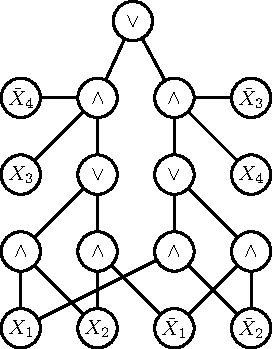
\includegraphics[width=0.65\linewidth]{figures/ddnnf}\vspace{-5pt}
        \begin{minipage}[t]{0.57\linewidth}
          \scriptsize \flushleft
          \textcolor{tractable_green}{\cmark \textbf{EVI}}, \textcolor{untractable_red}{\xmark \textbf{SAM}},
          \textcolor{tractable_green}{\cmark \textbf{MAR}},\par
          \textcolor{tractable_green}{\cmark \textbf{CON}},
          \textcolor{tractable_green}{\cmark \textbf{MPE}},
          \textcolor{tractable_green}{\cmark \textbf{Z}}
        \end{minipage}
      \end{center}
    \end{minipage}\begin{minipage}[t]{0.23\linewidth}
      \begin{center}
        \textbf{Sum-Product Networks}~\parencite{Poon2011}~($^{\times}$)\\[20pt]
        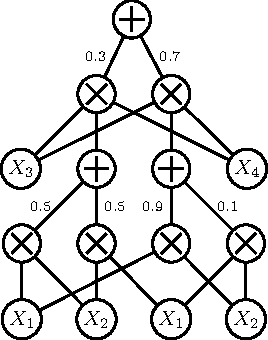
\includegraphics[width=0.55\linewidth]{figures/spn}\vspace{-10pt}
        \begin{minipage}[t]{0.48\linewidth}
          \scriptsize \flushleft
          \textcolor{tractable_green}{\cmark \textbf{EVI}}, \textcolor{tractable_green}{\cmark \textbf{SAM}},
          \textcolor{tractable_green}{\cmark \textbf{MAR}},\par
          \textcolor{tractable_green}{\cmark \textbf{CON}},
          \textcolor{untractable_red}{\xmark \textbf{MPE}},
          \textcolor{tractable_green}{\cmark \textbf{Z}}
        \end{minipage}
      \end{center}
    \end{minipage}\begin{minipage}[t]{0.19\linewidth}
      \begin{center}
        \textbf{NADEs}~\parencite{Larochelle2011}~($^{+}$)\\[20pt]
        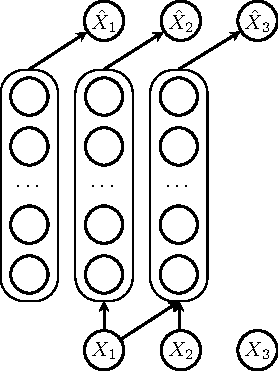
\includegraphics[width=0.63\linewidth]{figures/nade}\vspace{-5pt}
        \begin{minipage}[t]{0.57\linewidth}
          \scriptsize \flushleft
          \textcolor{tractable_green}{\cmark \textbf{EVI}}, \textcolor{tractable_green}{\cmark \textbf{SAM}},
          \textcolor{untractable_red}{\xmark \textbf{MAR}},\par
          \textcolor{untractable_red}{\xmark \textbf{CON}},
          \textcolor{untractable_red}{\xmark \textbf{MPE}},
          \textcolor{untractable_red}{\xmark \textbf{Z}}
        \end{minipage}
      \end{center}
    \end{minipage}\begin{minipage}[t]{0.19\linewidth}
       \begin{center}
         \textbf{MADEs}~\parencite{Germain2015}~($^{+}$)\\[20pt]
         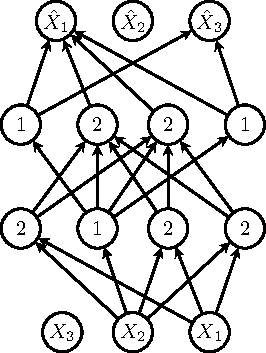
\includegraphics[width=0.63\linewidth]{figures/made}\vspace{-5pt}
         \begin{minipage}[t]{0.57\linewidth}
           \scriptsize \flushleft
           \textcolor{tractable_green}{\cmark \textbf{EVI}}, \textcolor{tractable_green}{\cmark \textbf{SAM}},
           \textcolor{untractable_red}{\xmark \textbf{MAR}},\par
           \textcolor{untractable_red}{\xmark \textbf{CON}},
           \textcolor{untractable_red}{\xmark \textbf{MPE}},
           \textcolor{untractable_red}{\xmark \textbf{Z}}
         \end{minipage}
      \end{center}
    \end{minipage}
    
  \end{textblock}
  
  %mixture
  % section 2
  \begin{textblock}{80}(0, 33.8)
    \usebeamerfont{section name}
    Representation Learning with TPMs
  \end{textblock}
  
  \begin{textblock}{25.2}(0, 36.3)
    \small
    \textbf{\emph{Representation Learning}} deals with generating new
    representations for the initial data $\{\mathbf x^i\}_{i=1}^m$,
    e.g. \textbf{\emph{embeddings}}
    $\{\mathbf{e}^i|\mathbf{e}^i\in\mathbb{R}^{k}\}_{i=1}^m $,
    $k$-dimensional continuous arrays.\par
    Once learned, one can employ them in new tasks such as
    supervised classification or
    clustering~\parencite{Bengio2012}.\\[20pt]

    Given a TPM $\theta$ we want to generate an embedding such as:
    $$\mathbf{e}^{i}=f_{p,\theta}(\mathbf{x}^{i})$$
    for each sample, with $f$ being a transformation provided by $\theta$ estimating the
    probability distribution $p$.\\[20pt]

    Simple idea: exploit the \emph{geometric space} induced by $p$,
    e.g. P-kernels, Fisher vectors\dots~\parencite{Shawe-Taylor2004},
    but:
    \begin{itemize}
    \item model dependent extraction
      \item closed form analytical derivation needed
    \end{itemize}
    
  \end{textblock}
  
  \begin{textblock}{25.2}(27.4, 36.3)
    \small
    We argue that TPMs can be employed as \emph{black box} embedding
    extractors, on a common ground, by answering generated templated
    queries.\\[20pt]

    We define two approaches exploiting a random query generator
    schema:
    \begin{enumerate}[I]
    \item templates are constructed by \textbf{random marginal
      queries}, i.e. generating subsets of r.v.s $\mathbf{Q}_{j} \subseteq
    \mathbf{X}, j = 1\dots,d$:
    $$e_{j}^{i}=p_{\theta}(\mathbf{Q}_{j}=\mathbf{x}^{i}_{\mathbf{Q}_{j}})$$
  \item generating a dataset of random \emph{patches} from samples,
    then training a TPM $\theta$ on it; embeddings are generated by evaluating $\theta$
    a sliding ``\emph{window}'' of size $d$ along the samples
    $$e_{j}^{i}=p_{\theta}(\mathbf{q}^{i}),\forall \mathbf{q}^{i}\sim \mathbf{x}^{i}, |\mathbf{q}^{i}|=d$$
  \end{enumerate}\bigskip

  Tractable inference is mandatory:
  for a congruous embedding size $k$, one has to perform $k\cdot
    m$ queries, e.g. on training split of BMNIST $k=10^{3},m=5\cdot
    10^{4}\rightarrow 5\cdot 10^{7}$ evals for approach I
  
  \end{textblock}



  % section 2.1
  \begin{textblock}{20}(54.8, 33.8)
    \usebeamerfont{section name}
    Experimental Design
  \end{textblock}

  \begin{textblock}{25.2}(54.8, 36.3)
    \small
    Planning an extensive experimentation comprising at least two TPMs
    from each family class, on a wide range of query types\\[20pt]
    
    Empirical evaluation of approach I on five binary image datasets
    used for classification:
    \begin{itemize}
    \item rectangles (\textsf{REC}), $28\times 28$ pixels, wide VS
      tall rectangles
    \item convex (\textsf{CON}), $28\times 28$ pixels, convex VS
      concave shapes
    \item ocr\_letters (\textsf{OCR}), $16\times 8$ pixels, ten digits
    \item caltech101 (\textsf{CAL}), $28\times 28$ pixels, 101 object shapes
    \item binary MNIST (\textsf{BMN}), $28\times 28$ pixels, ten
      digits
    \end{itemize}\vspace{15pt}
    
    Learning the structure of \emph{differently regularized} TPMs on RVs
    $\mathbf{X}$ alone (unsupervised) to compare different \emph{model capacities}:
    \begin{itemize}
    \item 3 SPN architectures trained with
      \textsf{LearnSPN-b}~\parencite{Vergari2015} with
      hyperparameters: $\rho=15$ for \textsf{OCR}
      and $\rho=20$ for all the rest, $m\in\{500,
      100, 50\}$  ($\rightarrow$ \textsf{SPN-I}, \textsf{SPN-II},
      \textsf{SPN-III}), then grid search on $\alpha\in\{0.1, 0.2,
      0.5, 1.0, 2.0\}$
    \item 3 Mixture of trees models (MT)~\parencite{Meila2000} with $k\in\{3,15,30\}$
      components ($\rightarrow$ \textsf{MT-I}, \textsf{MT-II},
      \textsf{MT-III}) trained with EM
    \end{itemize}\vspace{15pt}
    
    Extracting embeddings, then training a linear classifier on top of
    them to predict $Y$ (supervised):
    \begin{itemize}
    \item OVR L2-reg logistic regressor for all representations, grid
      search for regularization coefficient $C$ value in $\{0.0001, 0.001, 0.01, 0.1, 1.0\}$
      \item  baseline with initial representations ($\rightarrow$ \textsf{LR})
    \end{itemize}\vspace{15pt}

    
    Generating random queries:
    \begin{itemize}
    \item up to 1000 randomly generated marginal queries
      \item generating RVs over adjacent pixels in rectangular patches of min sizes of 2, max of 7 pixels for
      \textsf{OCR} and 10 pixels for the others
    \end{itemize}
  \end{textblock}

  
  %
  % section 3
  \begin{textblock}{80}(0, 59.6)
    \usebeamerfont{section name}
    Random query embedding extraction
  \end{textblock}
  
  
    
  \begin{textblock}{25.2}(0, 62.1)
    \small
    Approach I demands models for which marginals can be tractable
    \begin{itemize}
    \item more flexible: other kinds of inference kinds can be embedded,
      e.g. more complex query types~\parencite{Bekker2015}
    \end{itemize}
    \vspace{4pt}
    \begin{center}
      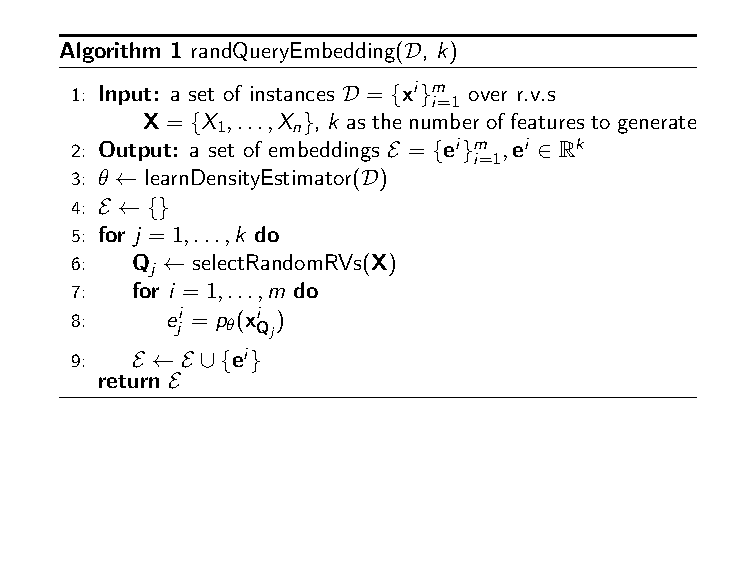
\includegraphics[width=0.9\linewidth]{algo_I}
    \end{center}

    % \footnotesize
    % % \begin{algorithm}[H]
    % %   \caption{\textsf{randQueryEmbedding}($\mathcal{D}$, $k$)}
    % %   \label{algo:randQuery}
    % \begin{algorithmic}[1]
    %   \State \textbf{Input:} a set of instances
    %   $\mathcal{D}=\{\mathbf{x}^{i}\}_{i=1}^{m}$ over r.v.s
    %   $\mathbf{X}=\{X_1,\dots,X_n\}$, $k$ as the number of features to generate
    %   \State  \textbf{Output:}  a set of embeddings
    %   $\mathcal{E}=\{\mathbf{e}^{i}\}_{i=1}^{m}, \mathbf{e}^{i}\in\mathbb{R}^{k}$
      
    %   \State $\theta\leftarrow\mathsf{learnDensityEstimator}(\mathcal{D})$
    %   \State $\mathcal{E}\leftarrow\{\}$
    %   \For {$j=1,\dots,k$}
    %   \State $\mathbf{Q}_{j}\leftarrow \mathsf{selectRandomRVs}(\mathbf{X})$
    %   \For {$i=1,\dots,m$}
    %   \State $e^{i}_{j}= p_{\theta}(\mathbf{x}^{i}_{\mathbf{Q}_{j}})$  
    %   \EndFor
    %   \State $\mathcal{E}\leftarrow\mathcal{E}\cup\{\mathbf{e}^{i}\}$
    %   \EndFor
    %   \Return {$\mathcal{E}$}
    % \end{algorithmic}
    % % \end{algorithm}

      \end{textblock}
  
      \begin{textblock}{25.2}(27.4, 62.1)
        \small
        % \footnotesize
        % % \begin{algorithm}[!t]
        % %   \caption{\textsf{randPatchEmbedding}($\mathcal{D}$, $s$, $d$)}
        % %   \label{algo:randPatch}
        % \begin{algorithmic}[1]
        %   \State \textbf{Input:} a set of instances
        %   $\mathcal{D}=\{\mathbf{x}^{i}\}_{i=1}^{m}$ over r.v.s
        %   $\mathbf{X}=\{X_1,\dots,X_n\}$,
        %   $s$ as the number of patches to extract,
        %   $d$ as the patch length,
        %   \State  \textbf{Output:}  a set of embeddings
        %   $\mathcal{E}=\{\mathbf{e}^{i}\}_{i=1}^{m}, \mathbf{e}^{i}\in\mathbb{R}^{k}$
        %   \State $\mathcal{R}\leftarrow\{\}$
        %   \For {$i=1,\dots,s$}
        %   \State $\mathbf{x}^{\mathsf{rand}}\leftarrow
        %   \mathsf{selectRandomSample}(\mathcal{D})$
        %   \State $\mathbf{r}^{i}\leftarrow
        %   \mathsf{extractRandomPatch}(\mathbf{x}^{\mathsf{rand}}, d)$
        %   \State $\mathcal{R}\leftarrow\mathcal{R}\cup\{\mathbf{r}^{i}\}$
        %   \EndFor
          
        %   \State $\theta\leftarrow\mathsf{learnDensityEstimator}(\mathcal{R})$

        %   \State $\mathcal{E}\leftarrow\{\}$
        %   \For {$i=1,\dots,m$}
        %   \State $j\leftarrow 0$
        %   \For {\textbf{each} patch $\mathbf{q}^{i}, |\mathbf{q}^{i}|=d$ in
        %     $\mathbf{x}^{i}$}
        %   \State $e^{i}_{j}= p_{\theta}(\mathbf{q}^{i})$
        %   \State $j\leftarrow j + 1$
        %   \EndFor
        %   \State $\mathcal{E}\leftarrow\mathcal{E}\cup\{\mathbf{e}^{i}\}$
        %   \EndFor
        %   \Return {$\mathcal{E}$}
        % \end{algorithmic}
        % % \end{algorithm}
        Approach II requires only tractable pointwise evidence
        \begin{itemize}
        \item largely employable: many more models can answer pointwise
          queries in a tractable way
        \end{itemize}
        \begin{center}
          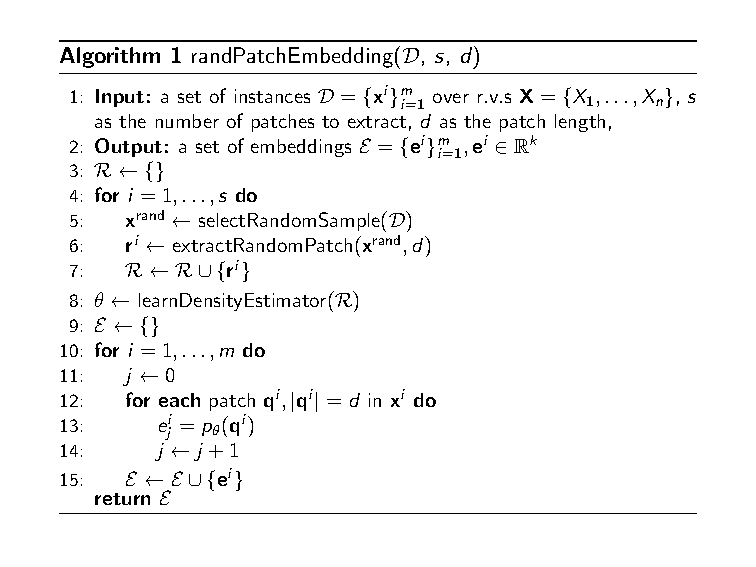
\includegraphics[width=0.9\linewidth]{algo_II}
        \end{center}
      \end{textblock}

      

      

      
  
  % 
  % section 5
  \begin{textblock}{80}(0, 82.9)
    \usebeamerfont{section name}
    Results
  \end{textblock}
  
  \begin{textblock}{25.2}(0, 85.4)
    \small
    For all models, less than $300$ features to beat the \textsf{LR}
    baseline\par
    \hspace{30pt}$\rightarrow$ the geometric space induced is meaningful/useful
  \end{textblock}
  
  \begin{textblock}{25.2}(27.4, 85.4)
    \small
    \textsf{SPN} embeddings outperform \textbf{MT} ones all datasets,
    but \textsf{CAL}\par
    \hspace{30pt}$\rightarrow$ MT scoring best likelihoods on
    $\mathbf{X}$ but worst accuracies for $Y$
  \end{textblock}
  
  \begin{textblock}{25.2}(54.8, 85.4)
    \small
    More regularized models perform better than specialized ones\par
    \hspace{30pt}$\rightarrow$ 
  \end{textblock}
  
  \begin{textblock}{80}(0, 89)
    \begin{center}
      \begin{minipage}[t]{0.2\linewidth}
        \begin{center}
          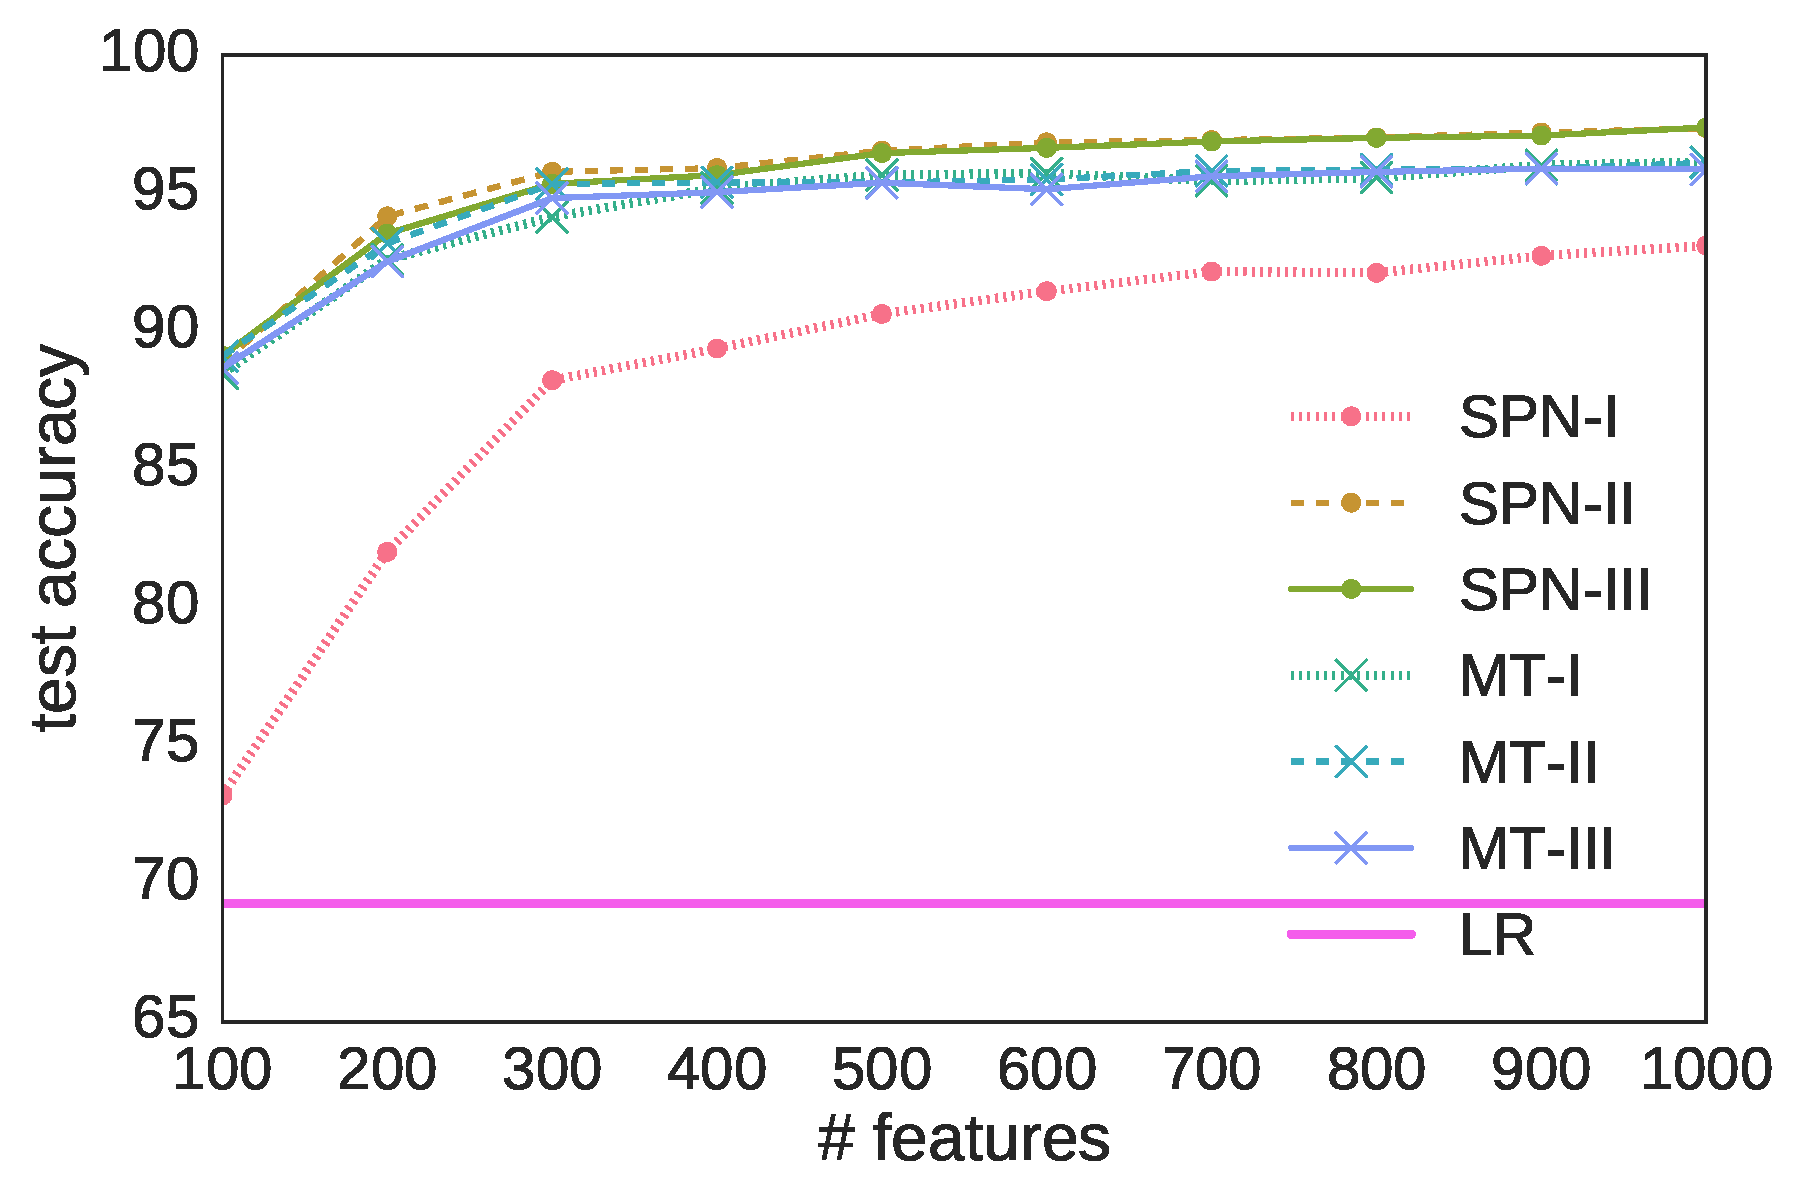
\includegraphics[width=1.0\linewidth]{figures/lines-rectangles}\par
          \footnotesize\textsf{REC}
        \end{center}
      \end{minipage}\begin{minipage}[t]{0.2\linewidth}
        \begin{center}
          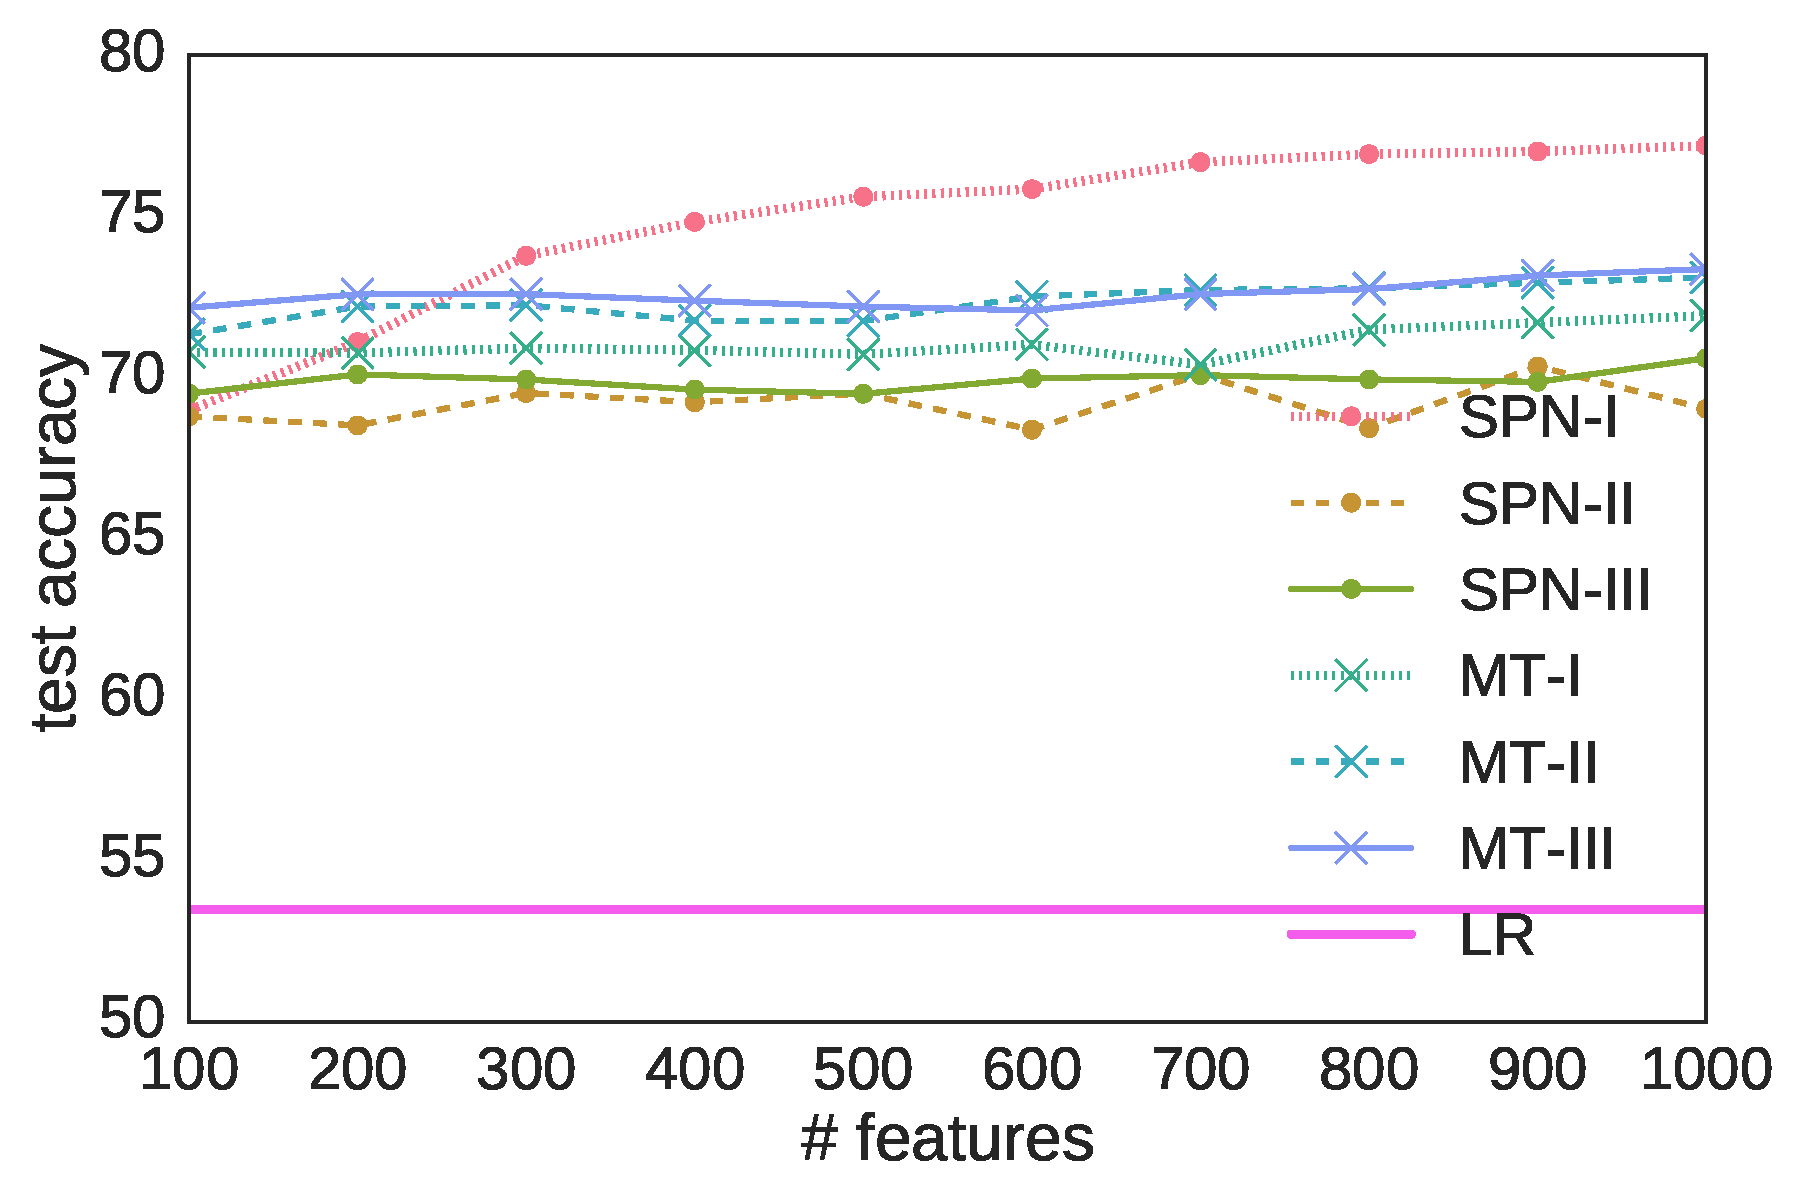
\includegraphics[width=1.0\linewidth]{figures/lines-convex}\par
          \footnotesize\textsf{CON}
        \end{center}
      \end{minipage}\begin{minipage}[t]{0.2\linewidth}
        \begin{center}
          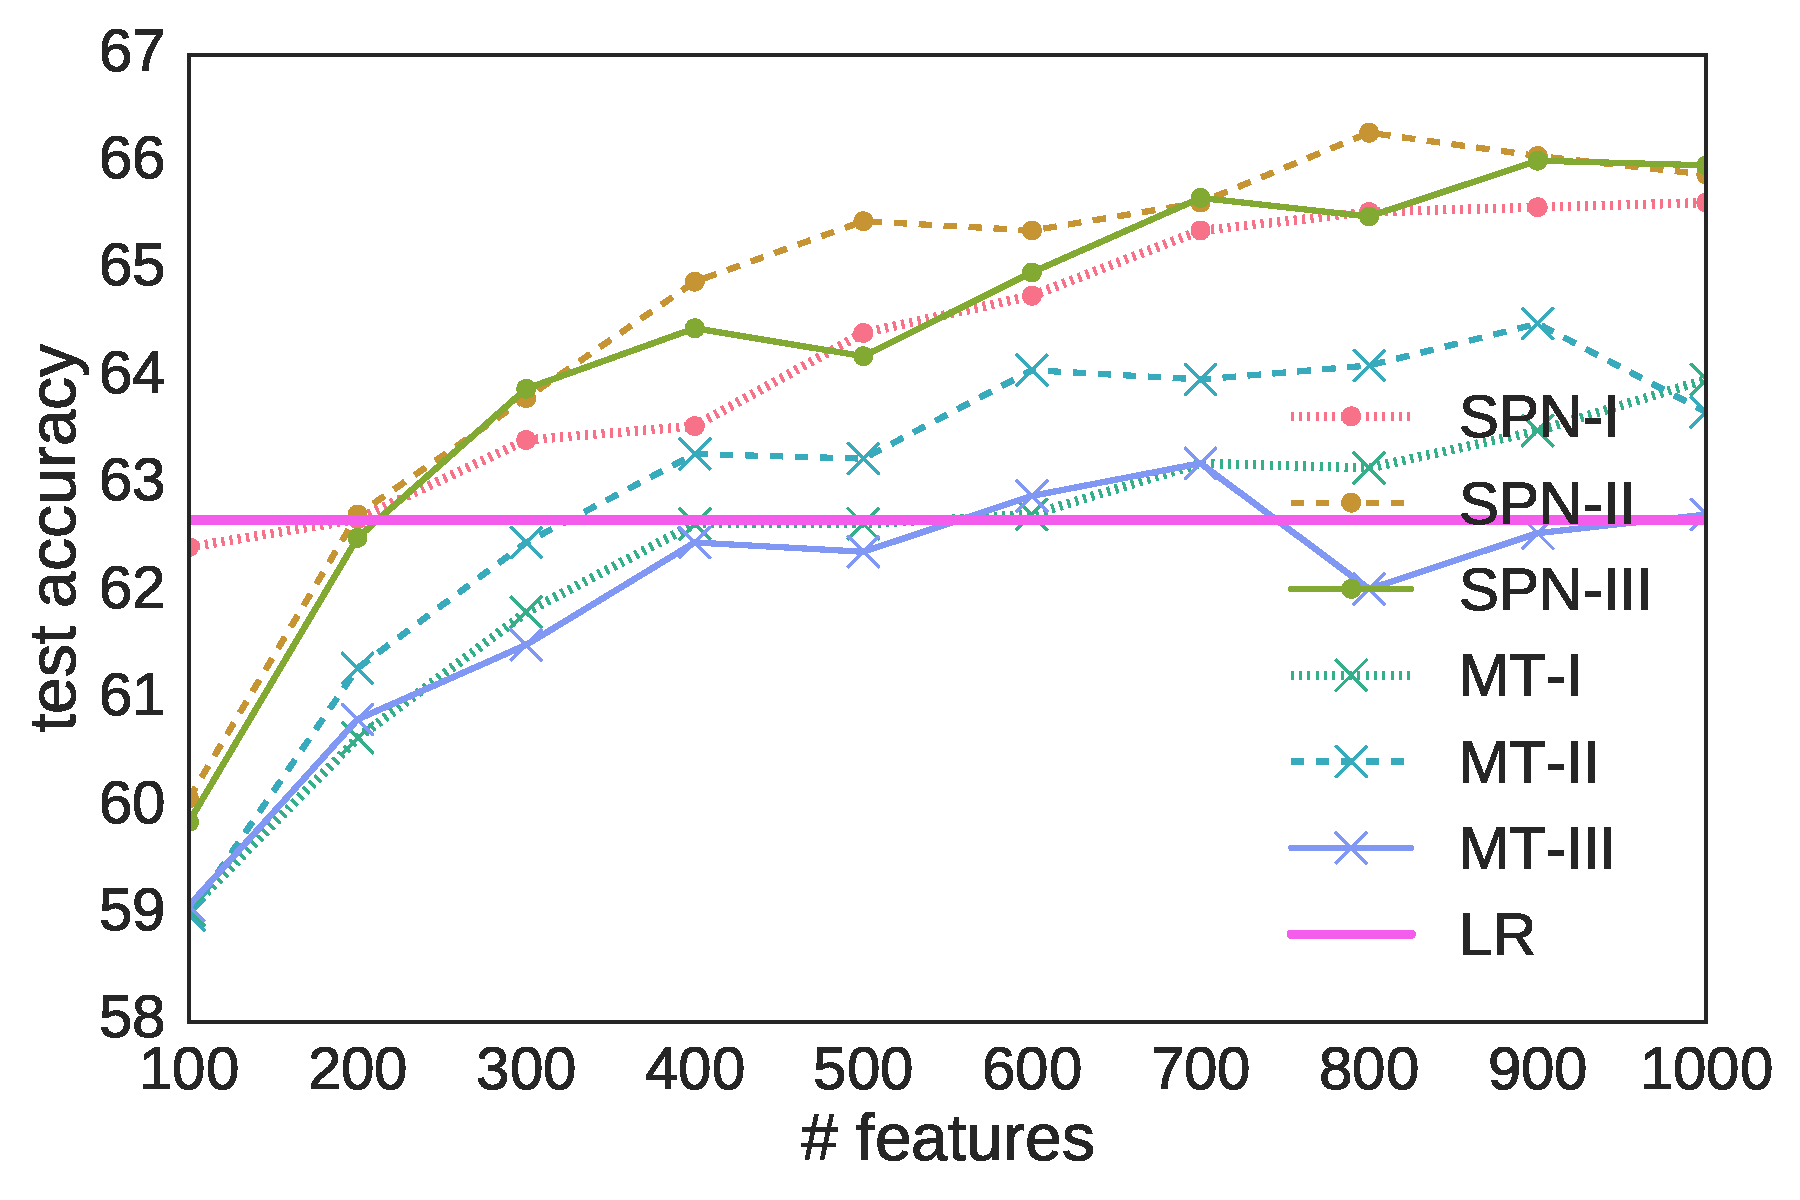
\includegraphics[width=1.0\linewidth]{figures/lines-caltech101}\par
          \footnotesize\textsf{OCR}
        \end{center}
      \end{minipage}\begin{minipage}[t]{0.2\linewidth}
        \begin{center}
          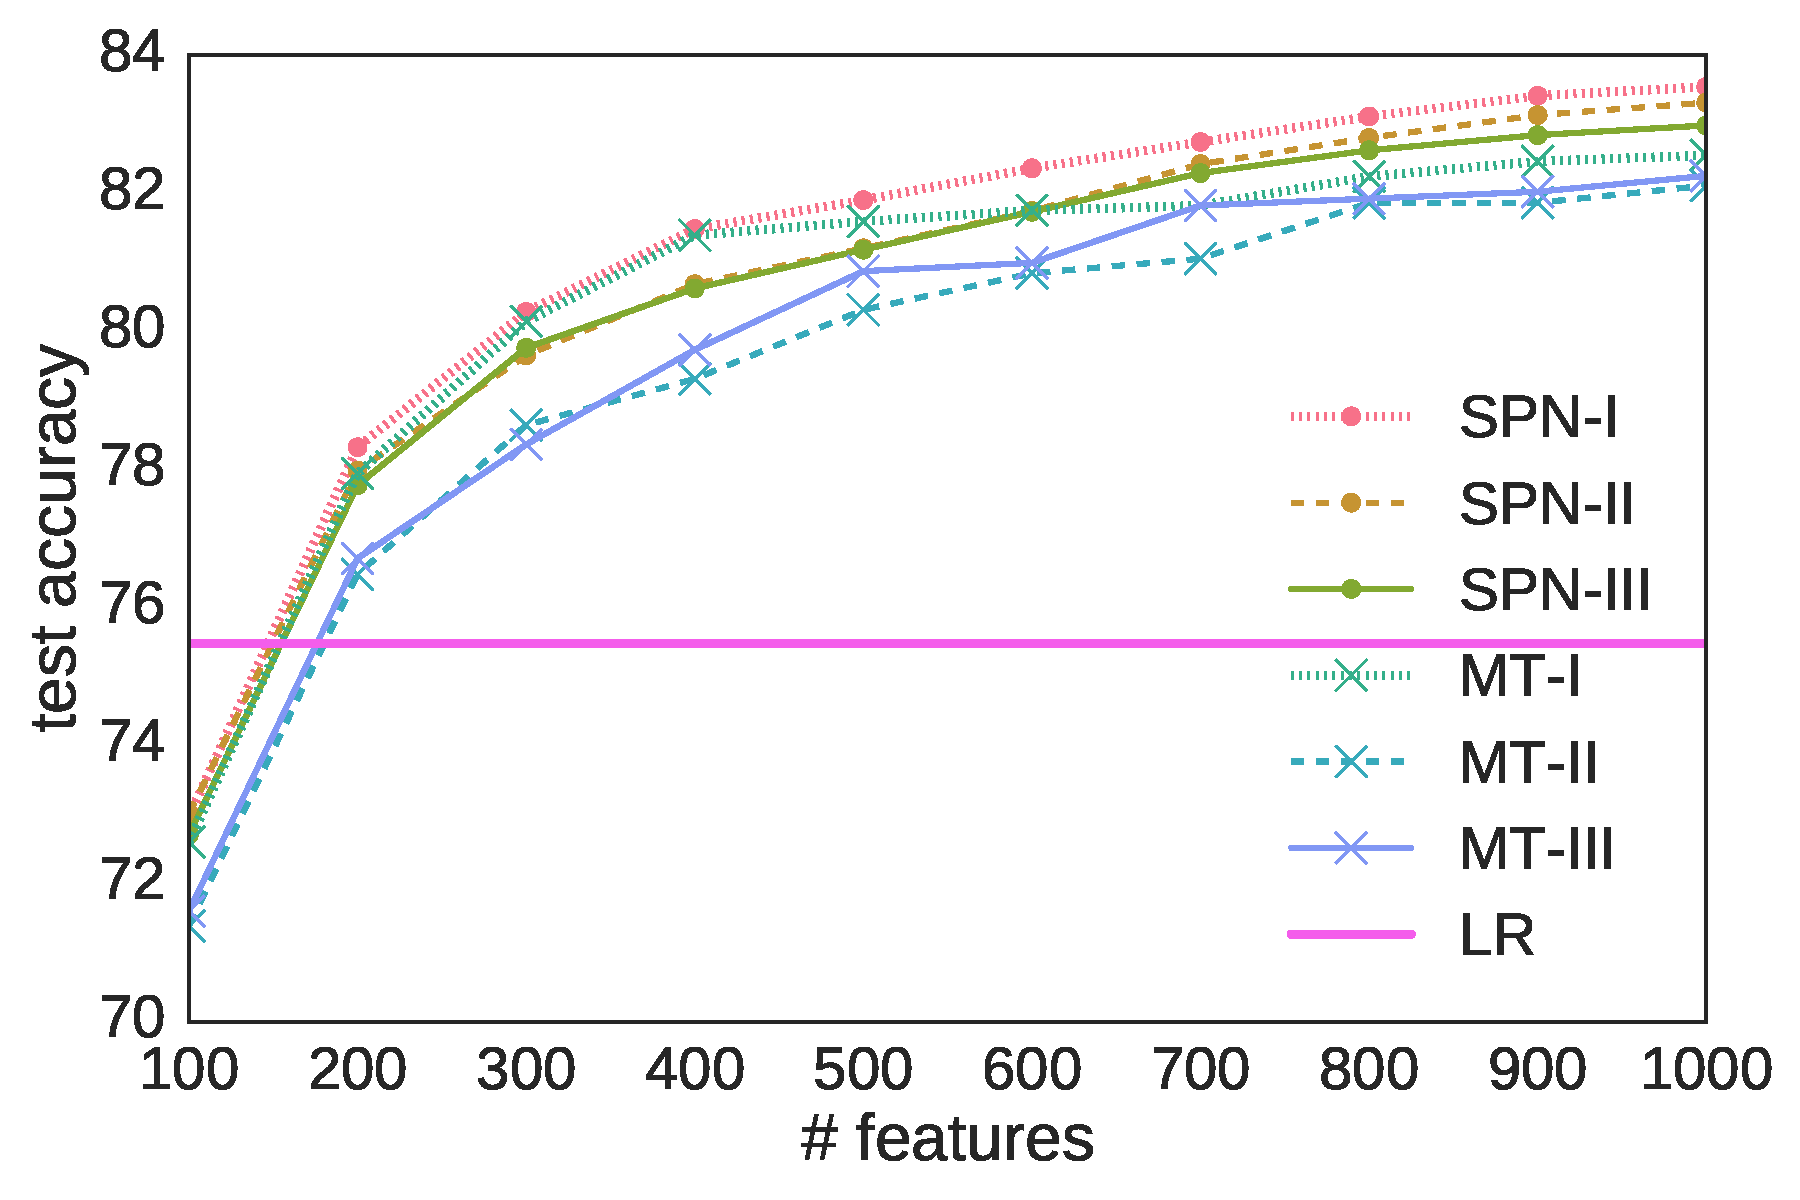
\includegraphics[width=1.0\linewidth]{figures/lines-ocr_letters}\par
          \footnotesize\textsf{CAL}
        \end{center}
      \end{minipage}\begin{minipage}[t]{0.2\linewidth}
        \begin{center}
          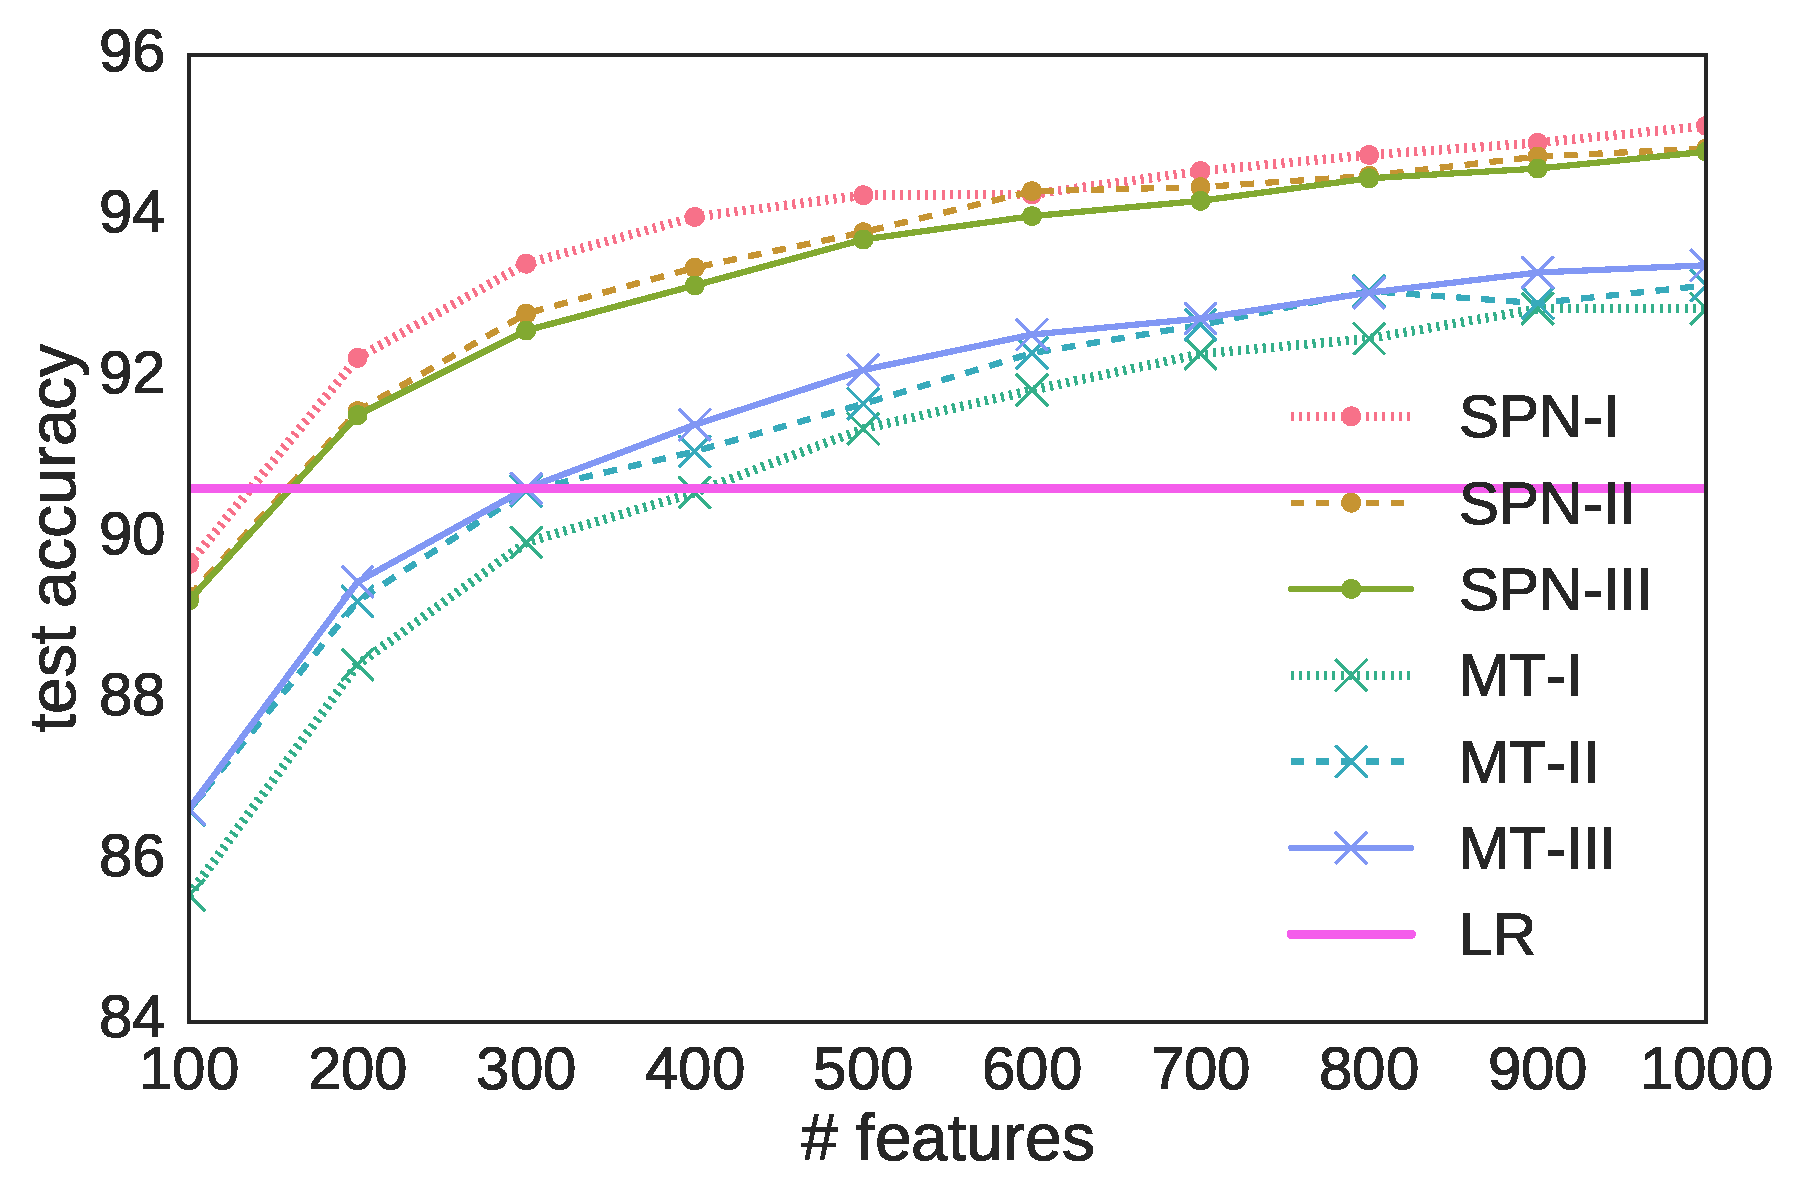
\includegraphics[width=1.0\linewidth]{figures/lines-bmnist}\par
          \footnotesize\textsf{BMN}
        \end{center}
      \end{minipage}
    \end{center}
  \end{textblock}
  
  % 
  % section 5
  \begin{textblock}{80}(0, 104.)
    \usebeamerfont{section name}
    References
  \end{textblock}

  \begin{textblock}{80}(54.8, 104.)
    \usebeamerfont{section name}
    Links
  \end{textblock}

  \begin{textblock}{52}(54.8, 106.5)
    \small
    paper available at:\par
    \hspace{35pt}\url{https://arxiv.org/abs/1608.02341}\\
    code available at:\par
    \hspace{35pt}\url{https://github.com/arranger1044/spyn-repr}\\
    more references:\par
    \hspace{35pt}\url{https://github.com/arranger1044/awesome-spn}
  \end{textblock}
  
 \begin{textblock}{52}(0, 106.5)
    \small
    % \blindtext
    \setlength\bibitemsep{8pt}
    \printbibliography[heading=none]
  \end{textblock}
  
  \begin{textblock}{25.2}(27.4, 106.5)
    \small
    % \blindtext
  \end{textblock}
  
  % \begin{textblock}{25.2}(54.2, 105.8)
  %   \small
  %   % \blindtext
  % \end{textblock}

  % 
  % footer
  \begin{textblock}{80}(0, 114.3)
    \usebeamerfont{subtitle}
    \footnotesize
    \flushright
    \textbf{ECML-PKDD 2016}  -  19th-23rd September 2016, Riva del Garda, Italy\hfill
  \end{textblock}
  
\end{frame}




\end{document}

%%% Local Variables:
%%% mode: latex
%%% TeX-master: t
%%% TeX-engine: xetex
%%% End:
